%=============================================================================
% Thesis Template in LaTex
%
% File: Sensitivitätsanalyse -- Fallstudie
% Author(s): Jürgen Hackl <hackl@ibi.baug.ethz.ch>
%            Clemens Kielhauser <kielhauser@ibi.baug.ethz.ch>
%
% Creation:  27 Jan 2014
% Time-stamp: <Tue 2013-08-13 20:14 juergen>
%
% Copyright (c) 2014 Infrastructure Management Group (IMG)
%               http://ibi.ethz.ch
%
% More information on LaTeX: http://www.latex-project.org/
%=============================================================================

% Unterkapitel Sensitivitätsanalyse
% ---------
\label{subsec:Sensitivitätsanalyse}

Wie im Abschnitt \ref{sec:Sensitivität} erläutert, wird mithilfe der Sensitivitätsanalysen, die in einem ersten Schritt ermittelte Lösung weiter untersucht, um die Belastbarkeit der Ergebnisse, in einer allfälligen Diskussion der Variante, zu stärken. Da auf die Phase der Erarbeitung einer Infrastruktur Intervention eine politische Diskussionen folgt, die den weiteren Verlauf des Projekts massgeblich bestimmt, ist eine vertiefte Untersuchung der Ergebnisse unerlässlich. Dies dient der Erabeitung einer Argumentationsbasis für die Verteidung der entwickelten optimalen Variante.

In diesem Schritt werden die Parameter der Risikoberechung verändert, die im Rahmen der politischen Auseinandersetzung das grösste Diskussionspotential bieten.
Die nachfolgenden Abschnitte umschreiben die durchgeführten Sensitivitätsanalysen und stellen die jeweiligen veränderten Parameter dar.

\paragraph{Zustand 0} untersucht der Grundzustand der Parameter und ist der Referenzwert der Sensitivitätsanalyse.

\paragraph{Zustand 1} Da der im Zustand 0 angenommene E-Auto Anteil eine progressive Prognosse ist, erachte ich eine differenzierte Untersuchung für angebracht. So simuliert der Zustand 1 eine konservative Prognosse des E-Auto Anteils im Jahr 2050 von 50\%. Wie in Abschnitt \ref{subsubsec:Marktanteil}, habe ich unter der Anahme eines linearen Wachstum, den in Abbildung \ref{img:Marktanteil-Z1} dargestellten jährlichen E-Auto Anteil \( \Phi_{E-Auto} \) berechnet. (\cite{Bestand2019})


\begin{figure}[h!]
	\centering
	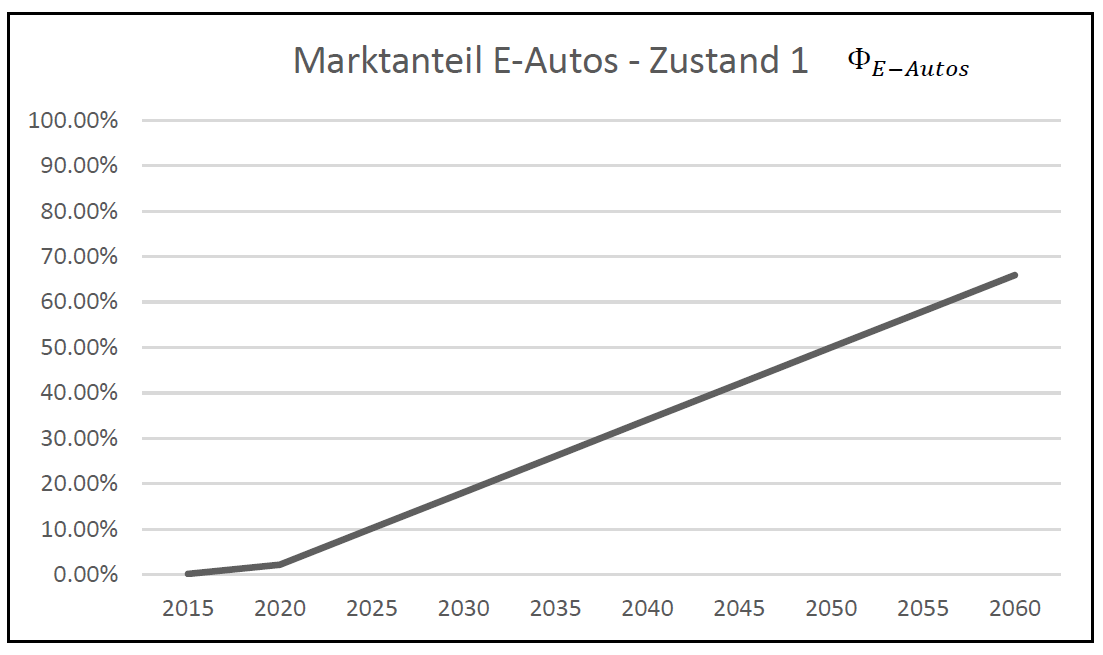
\includegraphics[width=.6\textwidth]{figures/f-04-09-01-Marktanteil-E-Autos-Zustand-1}
	\caption[Marktanteil E-Autos - Zustand 1]{Marktanteils der E-Autos am Strassenfahrzeugbestand - Zustand 1}
	\label{img:Marktanteil-Z1}
\end{figure}


\paragraph{Zustand 2} Da ich die Unfallwahrscheinlichkeiten anhand der gesamtschweizerischen Unfalldaten und Leistungen des Personenverkehrs berechne, erachte ich eine vertiefte Untersuchung dieser Parameter als notwenig. Um die effektive Gefahrenlage am Bahnübergang zu simulieren, verändere ich im Zustand 2 die Unfallwahrscheinlichkeiten. 

Um in der Variante 2 zu berücksichtigen, dass die erhöhte Durchfahrtsgeschwindigkeit in Verbindung mit der geringen Breite der Unterführung ein gewisses Sicherheitsrisiko darstellt, wird die Unfallwahrscheinlichkeit der Velofahrer um 50\% erhöht. \\
Im gleichen Schritt habe ich, unter der Annahme, dass die Einführung eines Ampelsystems und die dementsprechende einspurige Verkehrsführung, die Anzahl Unfälle auf dem Bahnübergang mit MIV-Beteiligung merklich reduziert sollte, die Unfallwahrscheinlichkeit des MIV wird in der Variante 3 demnach um 50\% gesenkt. 

Die ermittelten Unfallrisiken für den Zustand 2 sind in der nachfolgenden Tabelle zusammengefasst. 

%=============================================================================
% Thesis Template in LaTex
%
% File:  t-05-01-IsingModel.tex -- Table for the Ising
% Author(s): Juergen Hackl <hackl@ibi.baug.ethz.ch>
%            Clemens Kielhauser <kielhauser@ibi.baug.ethz.ch>
%
% Creation:  27 Jan 2014
% Time-stamp: <Tue 2013-08-13 20:14 juergen>
%
% Copyright (c) 2014 Infrastructure Management Group (IMG)
%               http://ibi.ethz.ch
%
% More information on LaTeX: http://www.latex-project.org/
%=============================================================================

\begin{table}[h!]
\scriptsize
\flushleft
\renewcommand{\arraystretch}{1.2} 
%
%
\begin{tabular}{@{} lccccccc @{}}  \\  
\toprule 
           & \multicolumn{2}{c}{\textbf{Unfalltyp\,a}} & \multicolumn{2}{c}{\textbf{Unfalltyp\,b}} & \multicolumn{2}{c}{\textbf{Unfalltyp\,c}} & Änderung  \\
           & MIV       & Velo      & MIV       & Velo      & MIV       & Velo    &  gegenüber Zustand 0 \\
\midrule
Variante 1&\(1.222\,\mathrm{10^{-7}}\)&\(1.117\,\mathrm{10^{-6}}\)&\(1.915\,\mathrm{10^{-8}}\)&\(3.484\,\mathrm{10^{-7}}\)&\(1.171\,\mathrm{10^{-9}}\)&\(1.032\,\mathrm{10^{-8}}\)& 0\% \\
Variante 2 &\(1.222\,\mathrm{10^{-7}}\)&\(1.676\,\mathrm{10^{-6}}\)&\(1.915\,\mathrm{10^{-8}}\)&\(5.226\,\mathrm{10^{-7}}\)&\(1.171\,\mathrm{10^{-9}}\)&\(1.548\,\mathrm{10^{-8}}\)& + 50\% für \(\gamma_{Velo,n}\)    \\
Variante 3 &\(5.853\,\mathrm{10^{-10}}\)&\(1.117\,\mathrm{10^{-6}}\)&\(9.576\,\mathrm{10^{-9}}\)&\(3.484\,\mathrm{10^{-7}}\)&\(6.108\,\mathrm{10^{-8}}\)&\(1.032\,\mathrm{10^{-8}}\)& - 50\% für \(\gamma_{MIV,n}\) 		\\
\bottomrule
\end{tabular}
\caption[Tabelle der Unfallrisiken - Zustand 2]{Tabelle der Unfallrisiken $\gamma_{j,n}\,\Bigl[\frac{Unf"alle_{j,n}}{Pkm_{j}}\Bigl]$ - Zustand 2}
\label{tab:t-09-01-Unfallrisiko-Zustand-2}
\end{table}





%=============================================================================
% EOF
%

%%% Local Variables:
%%% mode: latex
%%% TeX-master: "../guidelines"
%%% End:



\paragraph{Zustand 3} Die Eintrittswahrscheinlichkeiten im Zustand 0 habe ich anhand von Prognossen gesetzt. Um zu untersuchen welchen Effekt die Veränderung der Eintrittswahrscheinlichkeiten der Szenarien, auf die optimale Lösung hat, verändere ich im Zustand 3 die angenommen Eintrittswahrscheinlichkeiten. Die Eintrittswahrscheinlichkeit sind, wie in Abbildung \ref{img:EntscheidunSzenarien-Z3} ersichtlich, so verteilt, dass den Szenarien mit den grössten Wachstumsprognossen mehr Gewicht gegeben wird. 

\begin{figure}[h!]
	\centering
	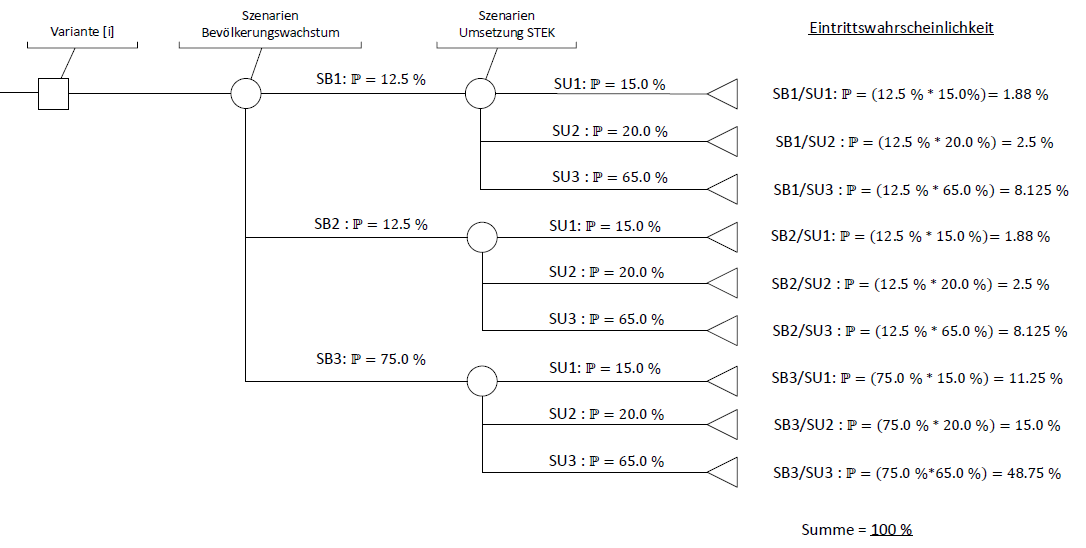
\includegraphics[width=\textwidth]{figures/f-04-09-02-Entscheidungsbaum-Szenarien-Zustand-3}
	\caption[Szenarienübersicht - Zustand 3]{Übersicht über die Szenarien und ihre Eintrittswahrscheinlichkeiten - Zustand 3}
	\label{img:EntscheidunSzenarien-Z3}
\end{figure}

\paragraph{Zustand 4} Um den Faktor Reisezeit genauer zu untersuchen und zu analysieren welchen Effekt die Veränderung der Reisezeit auf das Ergebniss hat, habe ich die prognostizierte durchschnittliche Wartezeit der Variante 3 wird von 7' auf 5' gesenkt, unter der Annahme, dass das eingeführte Ampelsystem zu keiner zusätzlichen Wartezeit führen wird.



% ===========================================================================
% EOF
%

%%% Local Variables:
%%% mode: latex
%%% TeX-master: "../main"
%%% End:
